\section{Mathematics Excursion III: Lagrange Multipliers and Extrema}

This is a lecture on the method of Lagrange multipliers, which essentially discusses optimization subject to constraints. We will use this perspective when discussing Lagrangian mechanics, so it's highly advised that one at least reads this particular set of notes through. In single-variable calculus, it's well-known how to optimize a function of a single variable, but this handout discusses how to do so with multiple variables, and with constraints imposed. 

\subsection{Extrema of Functions of Multiple Variables}
For this section, to begin with, we only discuss functions of two variables for visualization and simplicity. Of course, the techniques used here can be generalized easily. 

The most natural way to generalize the notion of a critical point for a function of multiple variables is by assuming \textit{all partial derivatives of a function $f$ with respect to all of its independent variables} at a critical point are zero or undefined, of which a function of only one variable gives us  a special case for this. This can equivalently be thought of saying that the gradient of this function, $\grad f$, is zero or undefined, which has some useful geometric intuition behind it. 

We can classify critical points based on the second derivatives of the variables. At a critical point, if the second (partial) derivatives of the function with respect to $x$ and $y$ are both positive, the function achieves a minimum, and similarly, if the second derivatives with respect to $x$ and $y$ are both negative, the function achieves a maximum. If one is positive and one is negative, we have what we call a \textit{saddle point}, which looks aptly like a saddle. This notion generalizes to functions of three or more variables, but obviously we can't see them as visually as we do here. 
\begin{figure}[h!]
\centering
\begin{minipage}{0.3\textwidth}
\centering
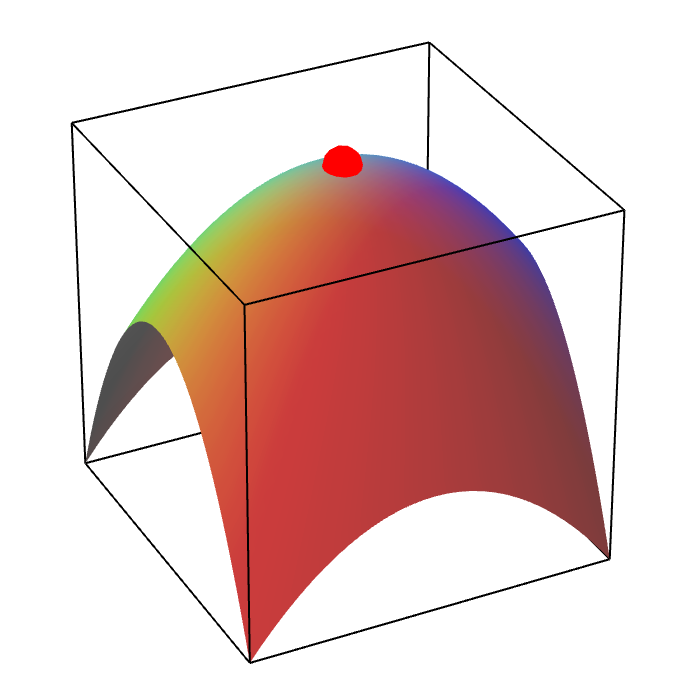
\includegraphics[scale=0.2]{images/math/multivar/localmax.png}
\end{minipage}
\begin{minipage}{0.3\textwidth}
\centering
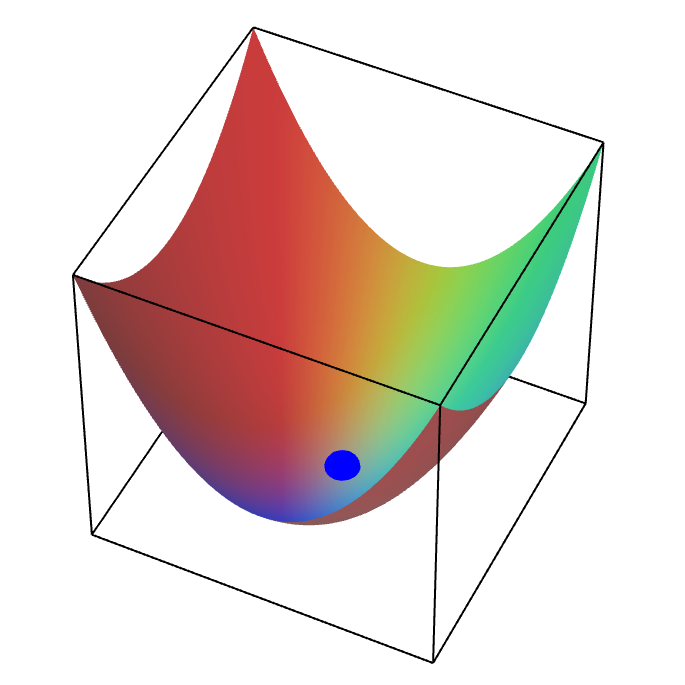
\includegraphics[scale=0.2]{images/math/multivar/localmin.png}
\end{minipage}
\begin{minipage}{0.3\textwidth}
\centering
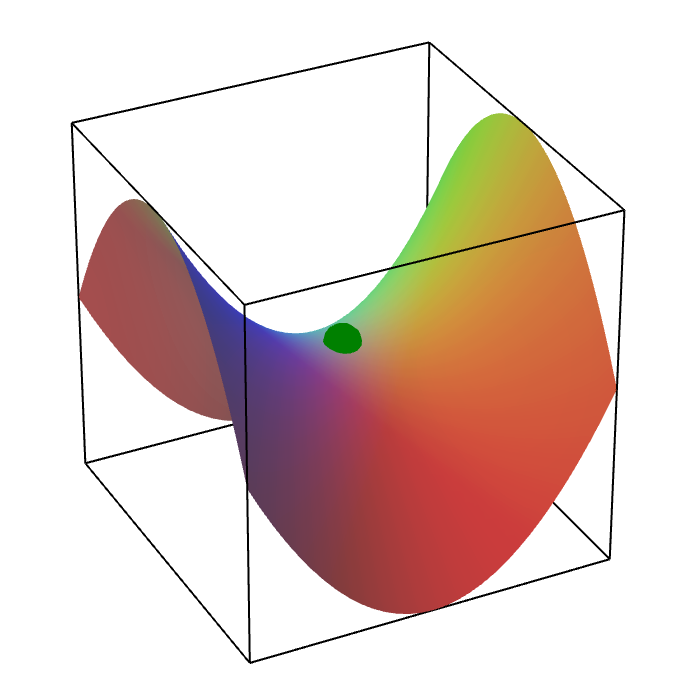
\includegraphics[scale=0.2]{images/math/multivar/saddlepoint2.png}
\end{minipage}
\end{figure}

%A theorem that we will now state for all multivariate functions, but not prove, is that on an open region, if a function is known to achieve a maximum or minimum value on the region, then it must do so at a critical point. 

\subsection{Optimizing with a Constraint}
Suppose now we want to optimize a function of two or more variables, but now subject to a constraint. Let's do an actual example for clarity: 
\begin{problem}
Find the maximum value of $x^3y$ on the ellipse $3x^2+2y^2 = 12$. 
\end{problem}
We can interpret this geometrically, first by considering the \textit{level curves} of the function we're studying (in this case, $f(x, y) = x^3y$), which are the curves of constant $f$. If we were to draw them out on top of the the ellipse on the plane, we can see that some sort of critical point should be reached when a level curve is tangent to the ellipse. If we think of the value of our constraint as a varying function $g(x, y) = 3x^2 + 2y^2$ that is forced to take on some value, this intuition tells us the gradients of these functions at this critical point should be parallel, ie. $\grad f = \lambda \grad g$ for some real $\lambda$. We call $\lambda$ the \textit{Lagrange multiplier} associated with $g$. Once we get the conditions associated with these parallel vectors, we can re-impose our constraint with $g$, and then get the desired maximum and the point at which the maximum is achieved. 

We could carry out the computation in this way, but we'll instead shift to a mostly algebraic/abstract way to do this that's equivalent. We'll incorporate the constraints and the function we're studying and roll them up into one function, what's sometimes called the \textit{Lagrangian function}. If our function of interest is $f$, and our constraints are $g$, we consider
\[
	\lagr(x, y) = f(x,y) + \lambda g(x, y).
\]
Conventionally, $g$ should be written in a form that should be equal to 0 when it is satisfied. We will take partial derivatives of $\lagr$ with respect to every independent variable and set them equal to 0 -- in this case, that would be $x$, $y$, and also $\lambda$. The partial derivative with respect to our Lagrange multiplier just gives back the constraint, and the other two equations will give a system of equations to solve. This will give us the proper critical points that we want. 

Let's actually do this example for real - let $\lagr(x, y) = x^3y - \lambda(3x^2 + 2y^2 -12)$, giving 
\[
	\lagr_x = 3x^2 y - 6 \lambda x = 0 \quad \lagr_y = x^3 - 4 \lambda y = 0 \quad \lagr_\lambda = 3x^2 + 2y^2 - 12 = 0 
\]
We more or less ignore the last equation until we use it as the constraint that needs to be satisfied, and we mess with the first two equations: 
\[
	6x^2 y^2 - 12\lambda x y - (3x^4 - 12 \lambda x y) = 3x^2(2y^2 - x^2) = 0
\]
Either $x = 0$, or from the constraint, $x^2 = 2y^2$ so $x = \pm \sqrt{3}$. We can now plug in each of these critical values of $x$ to see which one maximizes $x^3y$ (and by inspection, it's the value $x = \sqrt{3}$ with $y = \sqrt{\frac{3}{2}}$ that gives $\frac{9}{\sqrt{2}}$).
Notice that this latter perspective is much more generalizable, as it admits as many constraints. If we have $n$ constraints, each of which is a function $g_k$, we will instead consider the Lagrangian function 
\[
	\lagr(x, y) = f(x,y) + \sum_{k=1}^n \lambda_k g_k(x, y)
\]
and perform the same operations. 

The topic of Lagrangian multipliers and constrained optimization is important, and it will come up again when we discuss the Lagrangian method. 
